%%%%%%%%%%%%%%%%%%%%%%%%%%%%%%%%%%%%%%%%%
% Journal Article
% LaTeX Template
% Version 1.3 (9/9/13)
%
% This template has been downloaded from:
% http://www.LaTeXTemplates.com
%
% Original author:
% Frits Wenneker (http://www.howtotex.com)
%
% License:
% CC BY-NC-SA 3.0 (http://creativecommons.org/licenses/by-nc-sa/3.0/)
%
%%%%%%%%%%%%%%%%%%%%%%%%%%%%%%%%%%%%%%%%%

%----------------------------------------------------------------------------------------
%	PACKAGES AND OTHER DOCUMENT CONFIGURATIONS
%----------------------------------------------------------------------------------------

\documentclass{article}

%\documentclass{aastex}  % version 5.0 or prior
%\usepackage{natbib}



\usepackage{graphicx}
\usepackage{lipsum} % Package to generate dummy text throughout this template
%\usepackage[sc]{mathpazo} % Use the Palatino font
\usepackage[T1]{fontenc} % Use 8-bit encoding that has 256 glyphs
\linespread{1.05} % Line spacing - Palatino needs more space between lines
\usepackage{microtype} % Slightly tweak font spacing for aesthetics

\usepackage[margin=1in,columnsep=20pt]{geometry} % Document margins
\usepackage{multicol} % Used for the two-column layout of the document
\usepackage[hang, small,labelfont=bf,up,textfont=it,up]{caption} % Custom captions under/above floats in tables or figures
\usepackage{booktabs} % Horizontal rules in tables
\usepackage{float} % Required for tables and figures in the multi-column environment - they need to be placed in specific locations with the [H] (e.g. \begin{table}[H])
\usepackage{hyperref} % For hyperlinks in the PDF
\usepackage{subcaption}

\usepackage{lettrine} % The lettrine is the first enlarged letter at the beginning of the text
\usepackage{paralist} % Used for the compactitem environment which makes bullet points with less space between them
\usepackage{amsmath}
\usepackage{abstract} % Allows abstract customization
\renewcommand{\abstractnamefont}{\normalfont\bfseries} % Set the "Abstract" text to bold
\renewcommand{\abstracttextfont}{\normalfont\small\itshape} % Set the abstract itself to small italic text

\usepackage{titlesec} % Allows customization of titles
%\renewcommand\thesection{\Roman{section}} % Roman numerals for the sections
%\renewcommand\thesubsection{\Roman{subsection}} % Roman numerals for subsections
%\renewcommand\thesubsubsection{\Alph{subsubsection}} % Roman numerals for subsections
\titleformat{\section}[block]{\LARGE\scshape}{\thesection}{1em}{} % Change the look of the section titles
\titleformat{\subsection}[block]{\Large\scshape}{\thesubsection}{1em}{} % Change the look of the section titles
\titleformat{\subsubsection}[block]{\large\scshape}{\thesubsubsection}{1em}{} % Change the look of the section titles

\usepackage{fancyhdr} % Headers and footers
\pagestyle{fancy} % All pages have headers and footers
\fancyhead{} % Blank out the default header
\fancyfoot{} % Blank out the default footer
\fancyhead[C]{Montana State University \quad $\bullet$ \quad CSCI 466 Artificial Intelligence \quad $\bullet$ \quad Group 21} % Custom header text
\fancyfoot[RO,LE]{\thepage} % Custom footer text

\newcommand{\ve}[1]{\boldsymbol{\mathbf{#1}}}

\title{\vspace{-15mm}\fontsize{24pt}{10pt}\selectfont\textbf{CSCI 446 Artificial Intelligence \\[2mm] Project 4 Final Report} } % Article title
\date{\today}
\author{
\large
\textsc{Roy Smart} \and \textsc{Nevin Leh} \and \textsc{Brian Marsh}\\[2mm] % Your name
}


%----------------------------------------------------------------------------------------

\begin{document}

	\maketitle % Insert title
	\thispagestyle{fancy} % All pages have headers and footers
	\normalsize

	\section{Introduction}
	\section{The Racetrack Problem}
	\section{Value Iteration}
		\subsection{Description}
		\subsection{Implementation}
		\subsection{Experimental Design}
	\section{$Q$-Learning}
		\subsection{Description}
			\textit{Q-learning} is a model-free reinforcement learning method for determining optimal action-selection policies \cite{ai}. An agent using this method leverages a quantity known as the $Q$-value to derive the optimal action $a$ for each state $s$. The $Q$-value, $Q(s,a)$ describes the expected utility for every action in every state within the environment and is learned by the agent using temporal difference learning.
			An expression to calculate the $Q$-value is given by \cite{ai} as
			\begin{equation}
				Q(s,a) \leftarrow Q(s,a) + \alpha \left[ R(s) + \gamma \max_{a'} Q(s',a') - Q(s,a) \right]
				\label{ql}
			\end{equation}
			where $a$ is the action that was executed in state $s$ that resulted in state $s'$ and $R(s)$ is the reward function. The constants $\alpha$ and $\gamma$ are known respectively as the learning rate and the discount factor. Equation \ref{ql} is used as an update rule to adjust the value of $Q(s,a)$ for each action-state pair in every time trial undertaken by the agent. Using this simple update rule and $Q$-values initialized to zero for every action-state, an agent can learn how to navigate an environment.
		\subsection{Implementation}
			We based the design of our algorithm on the function \textsc{Q-Learning-Agent} described in Figure 21.8 of \cite{ai}. 
			The table of action values, $Q[s,a]$ and the tabel of frequencies, $N[s,a]$ were stored in six-dimensional arrays representing every possible position, velocity and acceleration in both spatial dimensions.
			
			The agent took an astonishingly long time to train. To lower the training time, we adopted strategy where the agent was started close to the finish line and trained until convergence. The starting line was then moved back by $m$ squares and then again trained until convergence. This process was repeated until the actual start line had been reached. In this way, our $Q$-Learning agent could be incrementally trained, without having to wait around for a few months to complete training.
			
			To further improve training, we assigned a penalty to hitting the wall. We understand that this breaks the rules of the assignment slightly, but the training time was too preventative. This behavior could indicate a problem with our $Q$-Learning algorithm.
			
			The traditional way to detect convergence in $Q$-Learning is to measure the rate of change of the $Q$-values across the table, and exit once the rate is sufficiently small. We did not adopt this approach as it would have been computationally expensive. We instead opted for a convergence test based off of a running average of the timesteps required for $n$ trials.
			
			The learning rate, $\alpha$ and the discount factor, $\gamma$ were tuned by hand. The tuned parameters are outlined in Table \ref{Q_params};
			
			\begin{table}
				\centering
				\begin{tabular}{|l|c|}
					\hline
					Parameter & Value \\ \hline
					Base Reward & -1.0 \\ 
					Wall Reward & -2.0 \\
					Finish Reward & 1.0 \\
					Learning Rate & $1 \times 10^{-7}$ \\
					Discount Factor & 0.9 \\
					$m$ & 2 \\ \hline
				\end{tabular}
				\caption{Table of tunable values for the $Q$-Learning agent}
				\label{Q_params}
			\end{table}
		\subsection{Experimental Design}
		
			For our experiments, we measured the average number of time steps for the $Q$-Learning agent vs. the number of time trials. This has the effect of showing the rate of convergence of the $Q$-Learning algorithm and describing the overall performance of the algorithm as track complexity increases.
		
	\section{Results}
		\subsection{L-Track}
			\subsubsection{Without Restart}
			
				\begin{figure}[h!]
					\centering
					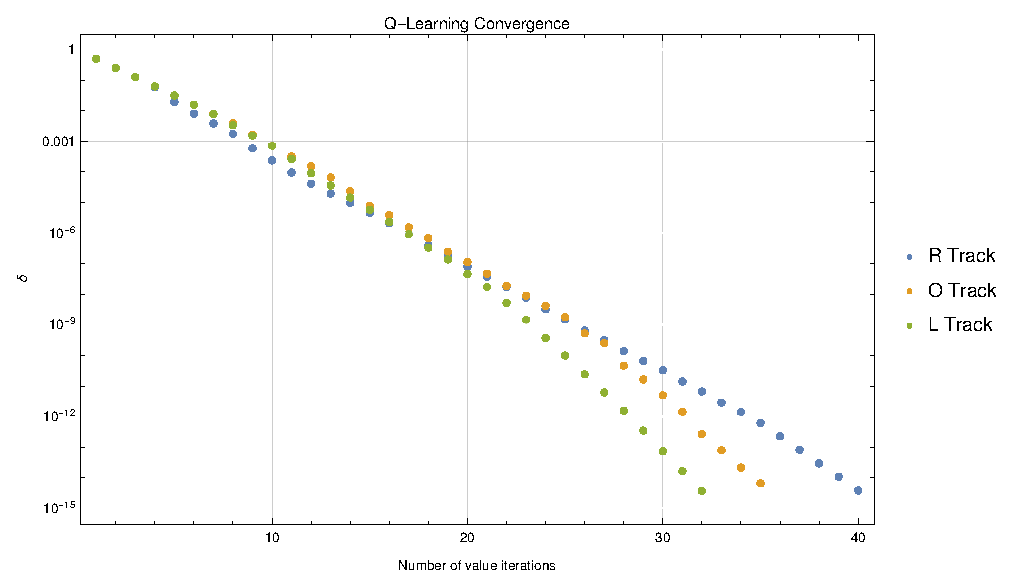
\includegraphics[width=0.8\textwidth]{Diagrams/VIter}
					\caption{}
					\label{VIter}
				\end{figure}
				
				
				
				\begin{figure}[h!]
					\centering
					\includegraphics[width=\textwidth]{Diagrams/QLearn}
					\caption{}
					\label{QLearn}
				\end{figure}
			
		\subsection{O-Track}
			\subsubsection{Without Restart}
		\subsection{R-Track}
			\subsubsection{Without Restart}
			\subsubsection{With Restart}
	\section{Conclusion}


	%\bibliographystyle{apj}
	\bibliographystyle{apalike}	
	\bibliography{sources}
\end{document}
